\documentclass{article}
\usepackage{tmlr}            % anonymized by default (loads natbib, fancyhdr)
\usepackage{amsmath,amssymb,amsthm}
\usepackage{graphicx}
\usepackage{booktabs}
\usepackage{microtype}
\usepackage[hidelinks]{hyperref}
\usepackage{url}

\newtheorem{theorem}{Theorem}
\newtheorem{proposition}{Proposition}

\title{Who, Not What: Identity Is Recoverable but Individual Behaviour Is Not\\
in Non-Invasive and In-Silico Neuroforecasting}

% Anonymized during review; author block is used only in the camera-ready.
\author{\name Anonymous \email anon@example.com \\
\addr Anonymous Institution}

\def\month{00}

\begin{document}
\maketitle

\begin{abstract}
A growing set of products and clinical tools claims to read an individual's mental state or behaviour
from brain and body signals, increasingly from a \emph{predicted} brain rather than a measured one: a
stimulus-to-cortex encoder maps media or context to cortical activity, which is then read as if it had
been recorded. We show that forecasting from a predicted brain obeys a simple structural limit, the
\emph{individuation gap}. Forecasting value separates into a population part and an individual part. The
population part improves with aggregation, which we prove, whereas the individual part depends on
between-subject variance that a zero-shot encoder does not carry, so it is zero without per-subject
enrollment. Three independent datasets show the consequence. Non-invasive readouts recover \emph{who} a
person is, with in-scanner fingerprinting at 100\% and a behavioural fingerprint at 14 times chance, but
not \emph{what} they will do, since the direct link from an individual's neural signal to that
individual's behaviour abstains under a calibrated test. A Bayes-optimal forecaster inherits the same
limit, adding no individual value at zero-shot and only a modest, saturating gain once per-subject data is
paid for. Combining signals does not remove the limit, because each added modality carries its own noise.
These results agree with the measurement-reliability literature, in which individual brain-behaviour
effects are small and require large samples, and they motivate a read-out that reports a value only when
it has earned the label. The contribution is a precise and verifiable account of what predicted-brain
readouts can and cannot deliver at the level of the individual.
\end{abstract}

\section{Introduction}
Imaging a brain and reading a mind are different acts, and the distance between them is easy to lose when a
model stands in for the scanner. Once an encoder maps a stimulus to a pattern of cortical activity, the
pattern can be labelled with the names that neuroscience gives to regions, and those labels can be sold as
measurements of attention, reward, or intent. The step from activity to label is reverse inference, and it
fails whenever a region serves more than one function, which is the usual case
\citep{poldrack2006,hutzler2013}.

Forecasting behaviour from \emph{measured} neural signals is, in contrast, a settled and useful idea.
Aggregate neural responses predict markets and audiences even when the sampled people's own choices do not
\citep{knutson2007,genevsky2017,dmochowski2014}, and the area has mature reviews of its methods
\citep{yao2024}. This paper concerns the move from a measured brain to a predicted one, and a property that
move forces into view. When the neural signal is itself a function of the stimulus, it can reproduce
whatever the stimulus already predicts while adding nothing of its own. Forecasting value then separates
into a population part and an individual part, and the two behave differently. The population part is
tractable and grows with aggregation; the individual part is bounded by the encoder and, for a person the
encoder never saw, is empty. We call this separation the individuation gap, state it as a theorem,
reproduce it on synthetic ground truth, and show that three real datasets fall where the gap predicts
(Figure~\ref{fig:overview}).

The question matters because the individual claim is the one being commercialised. Brand-intelligence
platforms, affective-computing products, and a new wave of personalized neuro-mental-health tools present an
individual readout, often from a predicted brain or from inexpensive peripheral signals, and present it as
a measurement of that person's state or likely behaviour. We ask whether that is achievable in principle by
non-invasive, in-silico means, and we find that it is not, in a sense we make precise. What such systems can
deliver is population forecasting and identity recognition, which are useful and real, and which should not
be confused with reading an individual's mental content.

\begin{figure}[t]
\centering
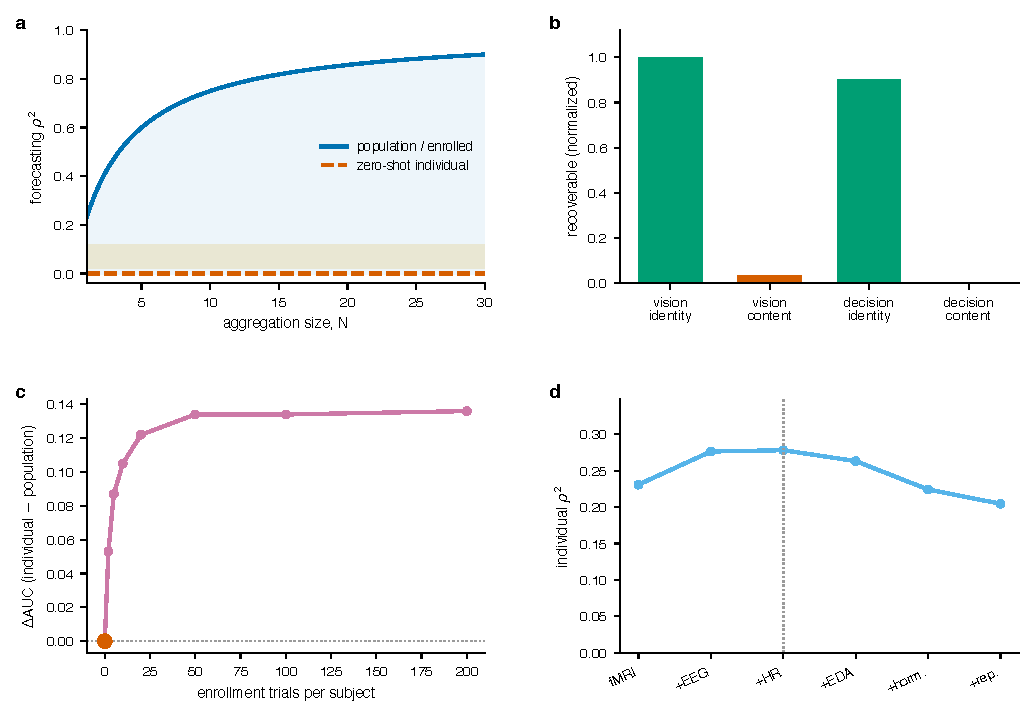
\includegraphics[width=0.92\textwidth]{../figures/fig0_overview.pdf}
\caption{\textbf{The individuation gap and its consequences.}
\textbf{(a)} Forecasting $\rho^2$ against aggregation size $N$ for the signal-plus-noise model of
Equation~\ref{eq:rho}. The population term (blue) rises with $N$; the zero-shot individual term (red) is
zero for all $N$. The shaded band marks the measured individual-difference ceiling reported for brain-wide
association studies ($r^2\approx0.02$ to $0.12$; \citealp{marek2022}).
\textbf{(b)} On real data, identity (who) is recoverable in both the vision-encoding and value-decision
settings, whereas individual behavioural content (what) is not; bars are normalized within each setting.
\textbf{(c)} A Bayes-optimal forecaster adds no individual value over the population model at zero-shot and
only a modest, saturating gain once per-subject trials are collected.
\textbf{(d)} Adding modalities is not free: each contributes signal but also noise, so individual $\rho^2$
rises then falls as lower-reliability signals are included.}
\label{fig:overview}
\end{figure}

\section{The individuation gap}
\label{sec:gap}
Let an outcome be $Y=S+\varepsilon$, where $\varepsilon$ is idiosyncratic noise of variance $v>0$ and $S$ is
the predictable component. Let the predictor resolve an identifiable signal variance $a\ge 0$, meaning the
between-unit variance it can actually recover. Taking the predictor to be $S$ in the best case gives
$\mathrm{Cov}(S,Y)=a$, $\mathrm{Var}\,S=a$, and $\mathrm{Var}\,Y=a+v$, so the best-case squared correlation
between predictor and outcome is
\begin{equation}
\rho^2(a,v)=\frac{a}{a+v}.
\label{eq:rho}
\end{equation}
Averaging the outcome over $N$ independent units replaces $v$ with $v/N$, the variance of a mean of $N$
independent terms, while leaving $a$ unchanged, which gives the population term $\rho^2(a,v/N)$. A zero-shot
encoder returns the same features for every unseen unit, so its predictor has no between-unit variance and
$a=0$.

\begin{theorem}[Population term]\label{thm:agg}
For $a,v>0$ and $N>1$, $\rho^2(a,v)<\rho^2(a,v/N)$.
\end{theorem}
\begin{theorem}[Zero-shot individual term]\label{thm:zero}
For every $v$ and $N$, $\rho^2(0,v/N)=0$.
\end{theorem}
\begin{theorem}[The gap]\label{thm:gap}
For $a,v>0$ and $N>0$, $\rho^2(0,v/N)<\rho^2(a,v/N)$.
\end{theorem}

The proofs are elementary: $\rho^2$ is strictly decreasing in the noise term, which gives
Theorem~\ref{thm:agg}; substituting $a=0$ into Equation~\ref{eq:rho} gives Theorem~\ref{thm:zero}; and the
two together give Theorem~\ref{thm:gap}. We machine-check all three in Lean~4 with Mathlib so that the limit
rests on a proof rather than on intuition; the theorem names and a listing are given in
Appendix~\ref{app:lean}.

Theorem~\ref{thm:zero} is the substantive statement. A predictor with no between-unit variance has zero
best-case correlation with the individual component of the outcome, at any noise level and for any amount of
pooling, because the quantity it would estimate is absent from its input. No increase in model quality
recovers it. This is the sense in which individual prediction from a zero-shot predicted brain is not merely
hard but unidentifiable.

\section{Identity is recoverable, behaviour is not}
\label{sec:whowhat}
If the individual term needs enrollment, the next question is what enrollment buys. Across three datasets it
buys identity rather than behaviour (Figure~\ref{fig:overview}b, Table~\ref{tab:real}).

Subject-specific image-to-fMRI encoders, fit on 7T data from eight people, encode held-out responses with
median correlations of $0.219$ to $0.463$. Cross-run fingerprinting then identifies the subject in all 25
regions tested at 100\% accuracy, against a chance rate of one in eight. The geometry that would carry
behaviourally relevant content is positive but small, between $0.005$ and $0.066$ across regions, and the
ceiling is set by the stimulus representation rather than by the training loss \citep{allen2022,chang2019}.
A value-based decision dataset tells the same story from the behavioural side. A phenotype built from 107
people and about 27{,}000 choices identifies individuals at 14 times chance ($p=5\times10^{-4}$) and predicts
held-out choices at an area under the curve of $0.965$, with conformal coverage of $1.00$ and an expected
calibration error of $0.034$; loss aversion recovers at $\lambda=1.45$, matching the original report
\citep{tom2007}, and the phenotype transfers between laboratories at $0.86$ to $0.89$. The population and
cross-laboratory links hold, yet the direct link from an individual's neural signal to that individual's
behaviour abstains under a calibrated minimum-detectable-effect test \citep{botviniknezer2019}. On the same
gambles, a content-only baseline already explains the aggregate, so a predicted neural index earns no
additional credit.

The pattern is consistent across modality and laboratory: the who question is answerable, the what question
is not. A system that treats the first as evidence for the second reports individual value it does not have.
The distinction is practical rather than semantic. Recovering identity supports verification and
personalization-by-lookup, which are legitimate functions; it does not support reading an individual's
current affect, intent, or next choice, which is the function most often advertised.

\begin{table}[t]
\centering\small
\caption{Convergent real-data evidence. Identity recovers in every setting; individual behavioural content
does not. Numbers are read from the corresponding analysis outputs (Appendix~\ref{app:data}).}
\label{tab:real}
\begin{tabular}{@{}lll@{}}
\toprule
Setting & Identity (who) & Behavioural content (what) \\
\midrule
Vision encoding (NSD, BOLD5000; $N{=}8$) & fingerprint 25/25 at 100\% & geometry $0.005$--$0.066$ (small) \\
Value decision (NARPS; $N{=}107$) & fingerprint 14$\times$ chance, $p{=}5{\times}10^{-4}$ & individual link abstains \\
Value decision, aggregate arm & population AUC $0.965$ & content baseline dominates \\
\bottomrule
\end{tabular}
\end{table}

\section{A Bayes-optimal forecaster inherits the limit}
\label{sec:bayes}
A principled probabilistic model does not rescue the individual where point estimates fail. In the zero-shot
regime a predictor with no between-subject variance is independent of the individual outcome given the
population, so the Bayes-optimal individual forecast equals the population forecast and the two share no
mutual information.

\begin{proposition}[Posterior collapse]\label{prop:bayes}
If the predictor is constant across subjects, the posterior over an individual's outcome equals the
population prior, and no estimator beats the population rate on the individual-specific component.
\end{proposition}
\noindent\emph{Proof sketch.} A constant predictor $X$ has $\mathrm{Cov}(X,Y)=0$ for any $Y$, so it carries
no information about the individual deviation $Y-\mathbb{E}[Y\mid\text{population}]$; conditioning on $X$
leaves the population posterior unchanged, and the mutual information $I(X;Y\mid\text{population})=0$.
\hfill$\square$

A Bayesian simulation bears this out (Figure~\ref{fig:overview}c; Appendix~\ref{app:sim}). With a latent
per-subject bias and a grid posterior updated from each subject's own choices, the recovery correlation at
zero-shot is $0.00$ and the incremental area under the curve over the population model is $0.000$. Enrollment
then pays off, with recovery rising to $0.58$, $0.86$, and $0.99$ at $2$, $10$, and $200$ trials and the
incremental area under the curve rising to about $0.05$, $0.11$, and $0.14$ before it flattens. Individual
prediction is therefore possible once per-subject data is collected, but it is modest and it saturates short
of certainty. The simulation also gives the practical reading of the enrollment price: tens to hundreds of
per-subject trials buy a single-digit gain in area under the curve, which is consistent with the hours of
per-subject data that precision neuroimaging requires \citep{gordon2017}.

\section{Combining signals does not remove the limit}
\label{sec:fusion}
A common response is to add signals: electroencephalography, heart rate, electrodermal activity, hormonal
assays. When sources are independent, inverse-variance fusion lowers variance, and the fused variance is at
most that of the best single source, a fact we also machine-check (Appendix~\ref{app:lean}). The gain erodes
because real sources are not independent and each one carries its own measurement noise.

\begin{proposition}[Fusion is not monotone]\label{prop:fusion}
With fused signal $A=\sum_m a_m$ and fused noise $v+\sum_m\delta_m$, where $\delta_m$ is the noise the
$m$-th modality adds, the individual correlation $\rho^2=A/(A+v+\sum_m\delta_m)$ rises when modality $m$ is
added if and only if $a_m/\delta_m$ exceeds the current signal-to-noise ratio $A/(v+\sum_{k<m}\delta_k)$. A
low-reliability modality lowers it.
\end{proposition}
\noindent\emph{Proof sketch.} Adding modality $m$ changes $\rho^2$ from $A/(A+v+D)$ to
$(A+a_m)/(A+a_m+v+D+\delta_m)$, where $D=\sum_{k<m}\delta_k$. Cross-multiplying, the new value exceeds the
old one exactly when $a_m(v+D)>A\delta_m$, that is when $a_m/\delta_m>A/(v+D)$. \hfill$\square$

Figure~\ref{fig:overview}d plots this. High-reliability sources help, and low-reliability ones, such as
single-channel autonomic measures or slow and state-dependent hormonal assays, push the individual
correlation back down. Fusion can raise the population term; it does not supply the between-subject signal
the individual term requires. The point is not that multimodality is useless but that it is governed by a
ratio, and that adding signals indiscriminately can reduce individual predictability rather than increase it.

\section{Why the individual level is hard}
\label{sec:reliability}
The gap is not a quirk of one pipeline. The measurement literature predicts it. Brain-wide associations have
small effect sizes, about $r=0.14$ for univariate and $r=0.34$ for multivariate methods, and require
thousands of participants to replicate, while within-person and interventional effects are larger
\citep{marek2022,kang2024}. Common task-fMRI measures of individual difference have poor test-retest
reliability, with a mean intraclass correlation of $0.397$, which caps their use as individual markers
\citep{elliott2020}; multivariate signatures can do better, which is the appropriate qualification rather
than a rescue \citep{kragel2021}. Individual precision mapping is achievable, but it takes hours of data per
person \citep{gordon2017,du2025}. Each of these is Equation~\ref{eq:rho} stated empirically: the individual
term is small and costly, and a zero-shot predictor pays none of the cost.

\section{A read-out that withholds by default}
\label{sec:protocol}
The practical consequence is a read-out that reports nothing unless three conditions hold
(Figure~\ref{fig:pipeline}). A construct score is returned only when the construct has a meta-analytic
localizer and its named regions are the best spatial match for its term, when the predicted index beats a
stimulus-only baseline out of sample, and when it carries a split-conformal interval \citep{vovk2005}.
Identity and content travel on separate channels, so a system may confirm who a person is without claiming
to read what they think. The specificity test alone withholds a persuasion index, because no localizer for
persuasion exists in the meta-analytic databases.

\begin{figure}[t]
\centering
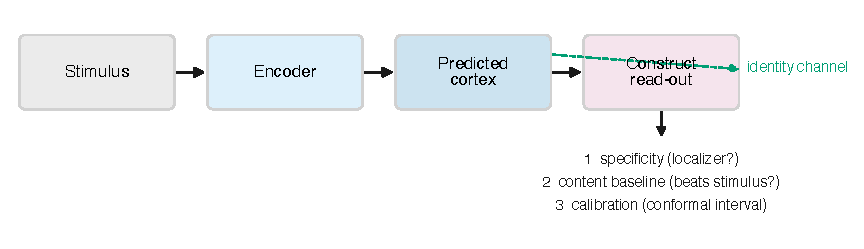
\includegraphics[width=0.9\textwidth]{../figures/fig_pipeline.pdf}
\caption{\textbf{A refusal-first read-out.} A predicted construct score passes only three gates in series:
a specificity gate (a validated localizer exists), a content-baseline gate (the index beats a stimulus-only
model), and a calibration gate (a conformal interval). Identity is reported on a separate channel from
content, so verifying a person does not imply reading their mental content.}
\label{fig:pipeline}
\end{figure}

\section{Validating the apparatus}
\label{sec:synthetic}
Before applying the control ladder to real data we checked that it recovers known truth on synthetic data
(Table~\ref{tab:gates}). We crossed a signal world, in which behaviour depends on an individual neural
component, with a null world, in which it depends only on content, and crossed both with an enrolled regime
(per-subject data) and an unseen regime (population-only features). Two preregistered tests ran on a nested
control ladder: a population test, correct subject against a capacity-matched non-brain basis, and an
individual test, correct subject against a wrong-subject permutation. The individual test fired in the one
cell where individual signal exists and the subject is enrolled, and stayed silent elsewhere, including both
null cells. The population test passed even in the null world, which is why it reports population value and
the individual test reports individual value. These numbers are synthetic; they check the method, not any
brain.

\begin{table}[t]
\centering\small
\caption{Synthetic apparatus check (20 seeds, paired bootstrap). The individual test fires only where
individual signal exists and the subject is enrolled.}
\label{tab:gates}
\begin{tabular}{@{}llll@{}}
\toprule
World / regime & Population test & Individual test & Expected \\
\midrule
Signal / enrolled & pass & pass, $+0.449$ [$+0.378,+0.526$] & fire \\
Signal / unseen & no & no, $+0.028$ & silent \\
Null / enrolled & pass, $+0.087$ & no, $-0.001$ & silent \\
Null / unseen & pass, $+0.034$ & no, $-0.001$ & silent \\
\bottomrule
\end{tabular}
\end{table}

\section{Reaching the individual level}
\label{sec:invasive}
The individual level is real and causally accessible, but at present only to invasive methods. Optogenetics
controls defined cell types and their effect on behaviour, and reads the brain-wide response when paired
with fMRI, in animals \citep{zhao2011,bernalcasas2017}. Intracortical interfaces decode attempted speech and
movement from one person's spiking activity at high accuracy and in daily home use
\citep{willett2023,card2025,silva2024}. These reach the individual because they record or perturb that
individual's own circuitry, which is exactly the between-subject signal a zero-shot non-invasive readout
lacks. They indicate where small individual signals may eventually be tracked, and they lie outside the
non-invasive consumer and clinical setting this paper concerns.

\section{Related work}
\label{sec:related}
Neuroforecasting from measured signals is established for anticipatory reward activity and for the temporal
reliability of evoked responses \citep{knutson2007,genevsky2017,dmochowski2014}, and reviews lay out its
theory and metrics \citep{yao2024}. The limits of inferring mental states from regional activity, and the
use of meta-analytic databases to quantify specificity, are long-standing \citep{poldrack2006,hutzler2013}.
Conformal prediction supplies distribution-free intervals with finite-sample coverage \citep{vovk2005}, and
a large literature quantifies the sample sizes and reliability needed for individual brain-behaviour
prediction \citep{marek2022,kang2024,elliott2020,kragel2021,gordon2017,du2025}. The field generally frames
the population-versus-individual distinction as a design trade-off to be managed with more data or better
estimators. Our contribution is to show that for a \emph{predicted} brain the distinction is a structural
boundary with a provable shape, that it is separate for identity and content, that it is not removed by
fusion, and that it can be enforced as a read-out protocol. We treat this as an account of what the setting
can and cannot support, in the spirit of studies that clarify the strengths and weaknesses of existing
methods, rather than as a new estimator.

\section{Discussion}
\label{sec:discussion}
The separation between a measured brain and a predicted one is not a matter of degree. A predicted readout
can report who a person is and can forecast a population, and it cannot report what an individual thinks or
will choose, because the individual signal is absent from its input until per-subject data is collected, and
that data currently buys identity more than behaviour. Fusion does not change this, a Bayes-optimal
forecaster does not escape it, and the reliability literature anticipated it. A readout built around the gap
returns fewer numbers, and the numbers it returns have earned their label.

Several limits of this account are worth stating plainly. The synthetic ladder and the Bayesian simulation
check the method and the probability claim, not any particular product. The three real-data results were
produced under separate analyses rather than one preregistered study, so they are convergent evidence rather
than a single confirmatory test, and the decision-fMRI individual link abstains at the edge of its power,
which is an abstention and not a positive null. The content-baseline comparisons are single-dataset. The
fusion result is an elementary consequence of the variance algebra beyond the independence lemma, and its
parameters in Figure~\ref{fig:overview}d are illustrative rather than measured. The model in
Equation~\ref{eq:rho} is a best-case linear-Gaussian abstraction; richer encoders change the constants but
not the sign of the gap, since $a=0$ for any zero-shot predictor. These are the boundaries within which the
claims hold.

\subsubsection*{Broader Impact Statement}
This work bears directly on products and clinical tools that claim to infer an individual's mental state or
behaviour from brain or body signals. Its central finding limits those claims: non-invasive and in-silico
readouts can recognize a person and can forecast populations, but cannot read an individual's mental content
without per-subject data, and even then only modestly. The positive impact is protective. A clear, provable
boundary and a refusal-first protocol give regulators, clinicians, and buyers a basis to reject overclaiming,
and give builders a standard that reports a value only when it is supported. A possible negative impact is
that the identity result, which we show is the part that does work, could encourage surveillance or
re-identification uses; we therefore separate identity from content explicitly and recommend that identity
recognition be treated with the privacy safeguards appropriate to biometrics. The work uses only existing,
de-identified public datasets and introduces no new data collection.

\section{Conclusion}
A predicted brain readout can tell you who someone is and can forecast a crowd. It cannot tell you what an
individual is thinking or will choose, because the individual signal is not in its input until per-subject
data is collected, and that data currently buys identity more than behaviour. We stated this as a theorem,
confirmed it on synthetic ground truth, showed three datasets fall where it predicts, and gave a read-out
that enforces it.

\bibliographystyle{tmlr}
\begin{thebibliography}{99}\small
\bibitem[Allen et al.(2022)]{allen2022} Allen, E.~J., et al. (2022). A massive 7T fMRI dataset to bridge cognitive neuroscience and artificial intelligence. \emph{Nature Neuroscience}, 25, 116--126.
\bibitem[Bernal-Casas et al.(2017)]{bernalcasas2017} Bernal-Casas, D., et al. (2017). Studying brain circuit function with dynamic causal modeling for optogenetic fMRI. \emph{Neuron}, 93(3), 522--532.
\bibitem[Botvinik-Nezer et al.(2019)]{botviniknezer2019} Botvinik-Nezer, R., et al. (2019). A large-scale fMRI dataset for the study of value-based decision making. \emph{Scientific Data}, 6, 106.
\bibitem[Card et al.(2026)]{card2025} Card, N.~S., et al. (2026). Long-term independent use of an intracortical brain--computer interface for speech and cursor control. \emph{Nature Medicine}, 32(7), 2504--2510.
\bibitem[Chang et al.(2019)]{chang2019} Chang, N., et al. (2019). BOLD5000: a public fMRI dataset of 5000 images. \emph{Scientific Data}, 6, 49.
\bibitem[Dmochowski et al.(2014)]{dmochowski2014} Dmochowski, J.~P., et al. (2014). Audience preferences are predicted by temporal reliability of neural processing. \emph{Nature Communications}, 5, 5567.
\bibitem[Du et al.(2025)]{du2025} Du, J.-N., et al. (2025). Within-individual precision mapping of brain networks exclusively using task data. \emph{Neuron}.
\bibitem[Elliott et al.(2020)]{elliott2020} Elliott, M.~L., et al. (2020). What is the test-retest reliability of common task-fMRI measures? \emph{Psychological Science}, 31(7), 792--806.
\bibitem[Genevsky et al.(2017)]{genevsky2017} Genevsky, A., Yoon, C., \& Knutson, B. (2017). When brain beats behavior: neuroforecasting crowdfunding outcomes. \emph{Journal of Neuroscience}, 37(36), 8625--8634.
\bibitem[Gordon et al.(2017)]{gordon2017} Gordon, E.~M., et al. (2017). Precision functional mapping of individual human brains. \emph{Neuron}, 95(4), 791--807.
\bibitem[Hutzler(2013)]{hutzler2013} Hutzler, F. (2013). Reverse inference is not a fallacy per se. \emph{NeuroImage}, 84, 1061--1069.
\bibitem[Kang et al.(2024)]{kang2024} Kang, K., et al. (2024). Study design features increase replicability in brain-wide association studies. \emph{Nature}, 636(8043), 719--727.
\bibitem[Knutson et al.(2007)]{knutson2007} Knutson, B., et al. (2007). Neural predictors of purchases. \emph{Neuron}, 53(1), 147--156.
\bibitem[Kragel et al.(2021)]{kragel2021} Kragel, P.~A., et al. (2021). Functional MRI can be highly reliable, but it depends on what you measure. \emph{Psychological Science}, 32(4), 622--626.
\bibitem[Marek et al.(2022)]{marek2022} Marek, S., et al. (2022). Reproducible brain-wide association studies require thousands of individuals. \emph{Nature}, 603, 654--660.
\bibitem[Poldrack(2006)]{poldrack2006} Poldrack, R.~A. (2006). Can cognitive processes be inferred from neuroimaging data? \emph{Trends in Cognitive Sciences}, 10(2), 59--63.
\bibitem[Silva et al.(2024)]{silva2024} Silva, A.~B., et al. (2024). The speech neuroprosthesis. \emph{Nature Reviews Neuroscience}, 25(7), 473--492.
\bibitem[Tom et al.(2007)]{tom2007} Tom, S.~M., et al. (2007). The neural basis of loss aversion in decision-making under risk. \emph{Science}, 315(5811), 515--518.
\bibitem[Vovk et al.(2005)]{vovk2005} Vovk, V., Gammerman, A., \& Shafer, G. (2005). \emph{Algorithmic Learning in a Random World}. Springer.
\bibitem[Willett et al.(2023)]{willett2023} Willett, F.~R., et al. (2023). A high-performance speech neuroprosthesis. \emph{Nature}, 620, 1031--1036.
\bibitem[Yao et al.(2024)]{yao2024} Yao, X., et al. (2024). Using neural data to forecast aggregate consumer behavior in neuromarketing. \emph{Journal of Consumer Behaviour}.
\bibitem[Zhao et al.(2011)]{zhao2011} Zhao, S., et al. (2011). Cell type-specific channelrhodopsin-2 transgenic mice for optogenetic dissection of neural circuitry function. \emph{Nature Methods}, 8(9), 745--752.
\end{thebibliography}

\appendix
\section{Lean formalization}
\label{app:lean}
The three statements of Section~\ref{sec:gap} and the inverse-variance fusion lemma of
Section~\ref{sec:fusion} are machine-checked in Lean~4 with Mathlib. We define
$\rho^2(a,v)=a/(a+v)$ and prove: \texttt{aggregation\_improves} (Theorem~\ref{thm:agg}),
\texttt{unseen\_individual\_is\_zero} (Theorem~\ref{thm:zero}), and \texttt{individuation\_gap}
(Theorem~\ref{thm:gap}); the fusion lemma \texttt{fused\_le\_min} states that the inverse-variance-fused
variance is at most that of any single source. The source is provided as supplementary material
(\texttt{IndividuationGap.lean}, \texttt{FusionMath.lean}).

\section{Simulation details}
\label{app:sim}
\textbf{Synthetic control ladder.} Data are generated under a crossed design: a signal world, in which the
outcome depends on an individual neural component, versus a null world, in which it depends only on content;
and an enrolled regime (leave-one-stimulus-out, so subjects recur) versus an unseen regime (held-out
subjects receive population-only features). Models are fit with ridge regression under cross-validated
regularization and scored by pooled out-of-sample $R^2$, with a paired bootstrap over 20 seeds. Gate~1
compares the correct-subject model against a capacity-matched non-brain basis; Gate~2 compares it against a
wrong-subject permutation.

\textbf{Bayesian enrollment.} Each subject $i$ has a latent bias $\theta_i\sim\mathcal{N}(0,s^2)$. On a trial
with stimulus value $x$, the choice probability is $\sigma(\beta x+\theta_i)$. A grid posterior over
$\theta_i$ is updated from the subject's enrollment choices. Individual value is measured two ways: the
correlation between the posterior-mean bias and the true bias, and the area under the curve of the enrolled
model minus the population model ($\theta=0$) on held-out trials. At zero-shot ($0$ enrollment trials) the
posterior equals the prior, $\hat\theta_i=0$ for all $i$, and both measures are zero by construction. Code
is provided as supplementary material (\texttt{prob\_falsification.py}).

\section{Data provenance}
\label{app:data}
Vision encoding uses the Natural Scenes Dataset and BOLD5000. Value-based decision uses NARPS (ds001734) and
ds000005. All reported statistics were read from the corresponding analysis outputs and should be
regenerated from a fixed commit for the camera-ready version. The reliability and intracortical-interface
figures are quoted from the cited papers.

\end{document}
